%
\documentclass[12pt,a4paper]{article}

\usepackage{epsfig}
\usepackage{hyperref}
\usepackage{graphicx}
\graphicspath{ {images/} }

\begin{document}
\begin{titlepage}
\title{Design Documentation\\CS Marks System\\ \small Version: 1.1}
\author{
Chris Moodley u10457489\\
Christo Brits u11080923\\
Christopher Crossman u10134842\\
Eduan Bekker u12214834\\
Mamelo Soepela u12094847\\
Z\"uhnja Riekert u12040593
}
\maketitle
\end{titlepage}
\tableofcontents
\pagebreak
\section{Software architecture design}
\subsection{Choices of Technologies}
\subsection{Chosen Frameworks}
\subsection{Chosen Protocols}
\subsection{Chosen Libraries}
\pagebreak
\section{Application design}
\subsection{Back-end System}
\subsection{Web Application}

\subsection{Android Application}
\subsubsection{Detailed System process specification}
All users need to enter a username and password when first opening the application on their android device.  This is necessary, for we do not want just anyone to be able to access the features and information that only specific users should have access to.\\\\
\textbf {Login:}
\begin{figure}[h]
\begin{center}
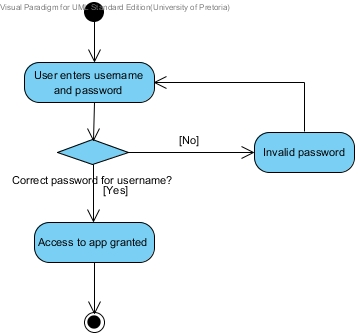
\includegraphics[scale=0.7]{ActivityDiagram1}
\end{center}
\end{figure}

After a user has gained access to the app, the user type (student/ teaching assistant/ lecturer) is detected.  The app only allows certain features to be available according to the user type\textquoteright s permissions.
\\

A student only has access to their own marks, thus when they choose to view marks, only their marks for the selected module are loaded. \\
\\
\textbf {Student views mark:}
\begin{figure}[h]
\begin{center}
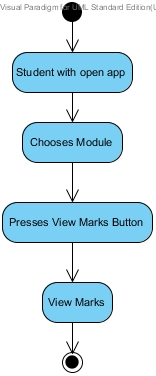
\includegraphics[scale=0.8]{ActivityDiagram2}
\end{center}
\end{figure} 

Students, like all users are however allowed to view the statistics for the selected module. \\
\\
\textbf {View statistics:}
\begin{figure}[h]
\begin{center}
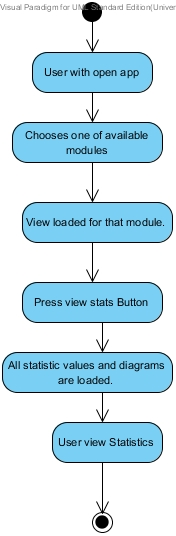
\includegraphics[scale=0.7]{ActivityDiagram3}
\end{center}
\end{figure}  

\newpage
\newpage
Both lecturers and TA’s should have the option to add marks for a student during the required specified time limit.\\
\\
\textbf {Adding marks:}
\begin{figure}[h]
\begin{center}
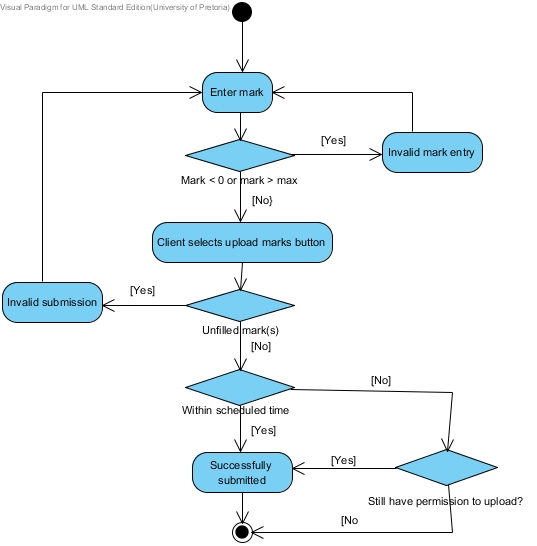
\includegraphics[scale=0.7]{ActivityDiagram5}
\end{center}
\end{figure}

\newpage
Only lecturers for a specific module should be able to edit marks after it has been uploaded.  Teaching will first need the permissions from the lecturer to be able to edit any marks.\\
\\
\textbf {Edit marks:}
\begin{figure}[h]
\begin{center}
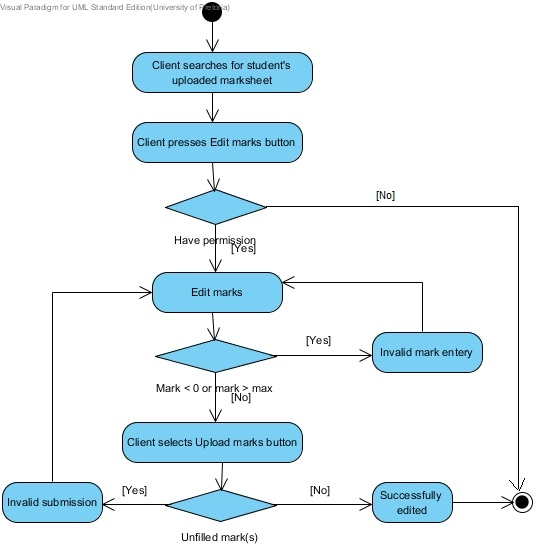
\includegraphics[scale=0.7]{ActivityDiagram6}
\end{center}
\end{figure}

\newpage
Only lecturers should be able to view all of the student's marks and give teaching assistants certain permissions.\\
\\
\textbf {Permissions and view all marks:}
\begin{figure}[h]
\begin{center}
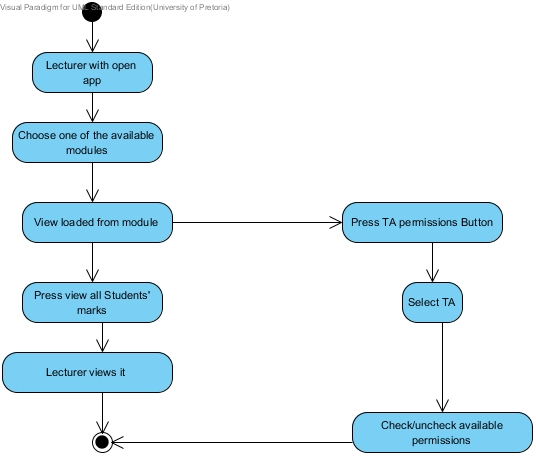
\includegraphics[scale=0.7]{ActivityDiagram4}
\end{center}
\end{figure}

\end{document}
